\chapter{Classificazione dei segnali}

\begin{figure}[h]
    \centering
    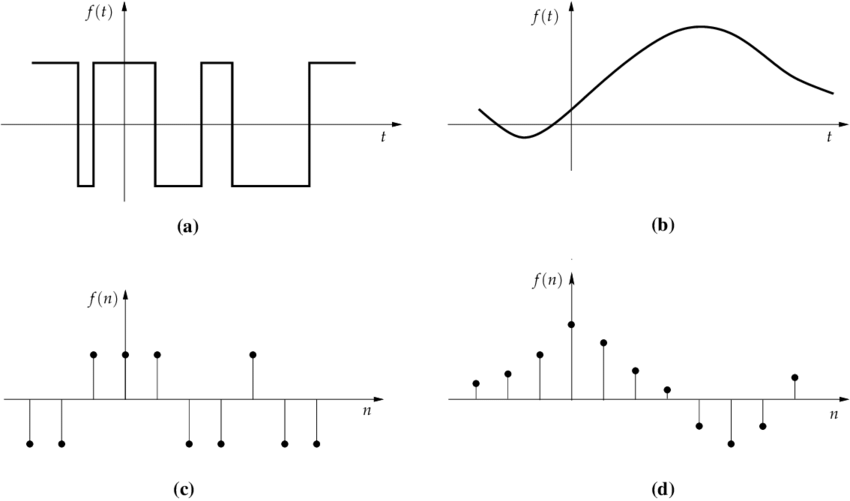
\includegraphics[scale = 0.5]{Figura-14-a-Segnale-a-valori-finiti-e-tempo-continuo-b-Segnale-continuo-a-tempo.png}
\end{figure}  

\newpage 

\section{Introduzione ai segnali} 

Per segnale si intende una funzione del tempo che rappresenta 
l'evoluzione temporale di una grandezza fisica. \newline 

Nel corso, per semplicità, saranno trattati come adimensionali, quindi senza grandezza fisica. \newline 

A partire dal segnale adimensionale, è possibile moltiplicarlo per una grandezza fisica, come ad esempio Volt o Ampere 
rispettivamente per un segnale in tensione e per un segnale in corrente. \newline 

I segnali, dal punto di vista macro, si dividono in due tipi: 

\begin{itemize}
    \item Segnali determinati 
    \item Segnali aleatori 
\end{itemize}


I segnali, sia aleatori che determinati, 
sono funzioni che possono essere a valori reali e/o a valori complessi. \newline 

Le funzioni sono continue e limitate. \newline 

I segnali determinati sono quei segnali in cui si conosce a priori il loro andamento temporale, 
quindi possiamo esplicitare il loro andamento per ogni t che va da $t = \infty$ a $t = -\infty$: 
questi segnali sono studiati grazie alla Teoria dei segnali. \newline 

Invece, i segnali aleatori sono quei segnali in cui non si conosce esplicitamente il loro andamento temporale, 
bensì, si utilizzano i concetti della Teoria della probabilità, per capire a priori la probabilità che un segnale possa essere in certi intervalli. \newline

Un segnale determinato non porta informazione perchè non ha alcuna incertezza a priori: \newline
esso è semplicemnte noto per qualunque instante di tempo. \newline 

Per essere informativo, il segnale non deve essere noto a priori. \newline 

L'obbiettivo dei sistemi di telecomunicazioni è quello di inviare informazioni, quindi soprattutto i segnali aleatori. \newline 

I segnali possono essere classificati in base alla loro variabile indipendente (generalmente il tempo) 
e alla loro grandezza che rappresentano (quindi l'ampiezza): 

\begin{itemize}
    \item Seganli a tempo continuo ed ampiezza continua 
    \item Segnali a tempo continuo ed ampiezza discreta 
    \item Segnali a tempo discreto ed ampiezza continua 
    \item Segnali a tempo discreto ed ampiezza discreta  
\end{itemize} 


\begin{figure}[h]
    \centering
    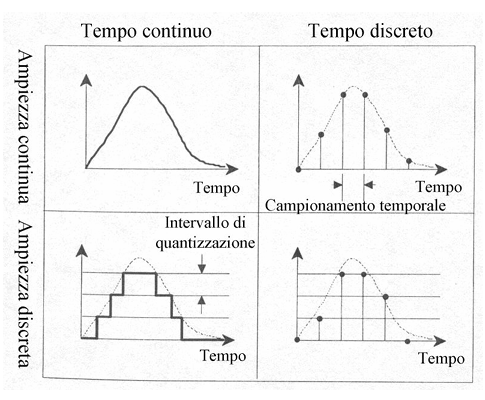
\includegraphics[scale = 0.8]{Classificazione segnali.PNG}
\end{figure}  

I segnali a tempo continuo ed ampiezza continua sono detti analogici e sono associati a fenomeni naturali (come un'onda acustica). \newline 

I segnali in cui le ampiezze sono discrete sono segnali in cui si è svolta l'operazione di quantizzazione, 
in cui il segnale reale analogico è stato trasformato in un numero. \newline 

Se anche il tempo è discreto, si definisce il segnale come digitale, che è comunemente impiegato nei sistemi digitali come i computer, microprocessori, ecc... \newline

Il processo di discretizzazione del tempo è detto campionamento. \newline 

\newpage

\section{Segnali periodici: cosa sono e quali sono i parametri utili}

I segnali periodici sono segnali che si ripetono in ogni intervallo T. \newline 

T prende il nome di periodo del seganle. \newline 

In formule matematiche, un segnale è periodico se $\forall t \in [-\infty, +\infty]$: 

{
    \Large 
    \begin{equation}
        s(t + T) = s(t)
    \end{equation}
}

Un esempio di segnale periodico: 

\begin{figure}[h]
    \centering
    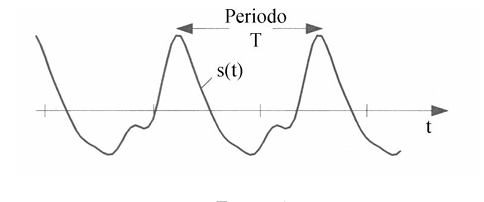
\includegraphics[scale = 0.8]{Esempio di segnale periodico.PNG}
\end{figure}  


Inoltre, viene definito come frequenza fondamentale $f_0$ l'inverso di T, cioè: 

{
    \Large 
    \begin{equation}
        f_0 = \frac{1}{T}
    \end{equation}
}

Generalmente t viene misurato in secondi, mentre la frequenza in Hertz: 

{
    \Large
    \begin{equation}
        [Hz] = \frac{1}{s}
    \end{equation}
}

In questo corso si predilisce utilizzare la pulsazione. \newline 

Si definisce la pulsazione fondamentale come: 

{
    \Large 
    \begin{equation}
        \omega_0 = 2\pi f_0
    \end{equation}
} 

e si misura in radianti al secondo: 

{
    \Large 
    \begin{equation}
        [\omega_0] = \frac{rad}{s}
    \end{equation}
}

Se il segnale è a tempo discreto, si predilisce utilizzare le parantesi quadre. \newline 

Se il segnale a tempo discreto è periodico, lo si può scrivere come: 

{
    \Large 
    \begin{equation}
        s[n + N] = s[n]
    \end{equation}
}

dove N è un numero intero. \newline 


Dato un segnale s(t) è possibile definire il suo valore medio temporale come: 

{
    \Large 
    \begin{equation}
        \overline{s(t)} 
        = 
        \lim_{\Delta T \rightarrow \infty} 
        \frac{1}{\Delta T}
        \int_{- \frac{\Delta T}{2} }^{\frac{\Delta T}{2} } 
        s(t) dt
    \end{equation}
}

In un segnale periodico: 

{
    \Large
    \begin{equation}
        \Delta T = kT
    \end{equation}
} 

Svolgendo alcuni passaggi algebrici che trovate nelle dispense del prof, avremo che: 


{
    \Large 
    \begin{equation}
        \overline{s (t)}
        = 
        \frac{1}{T} \int_{-\frac{T}{2}}^{\frac{T}{2}} 
        s(t) dt
    \end{equation}
}

Questa equazione è anche ovvia per definizione perchè, essendo un segnale periodico, se si conosce 
il suo valore medio temporale nel periodo T, lo si conosce $\forall T \in [-\infty, +\infty]$

\newpage 

\section{Delta di Dirac} 

La delta di Dirac è un impulso matematico definita come: 

{
    \Large 
    \begin{equation}
        \delta (t) 
        = 
        \lim_{\Delta t \rightarrow 0} 
        \frac{1}{\Delta t} rect_{\Delta t} (t)
    \end{equation}
}

\begin{figure}[h]
    \centering
    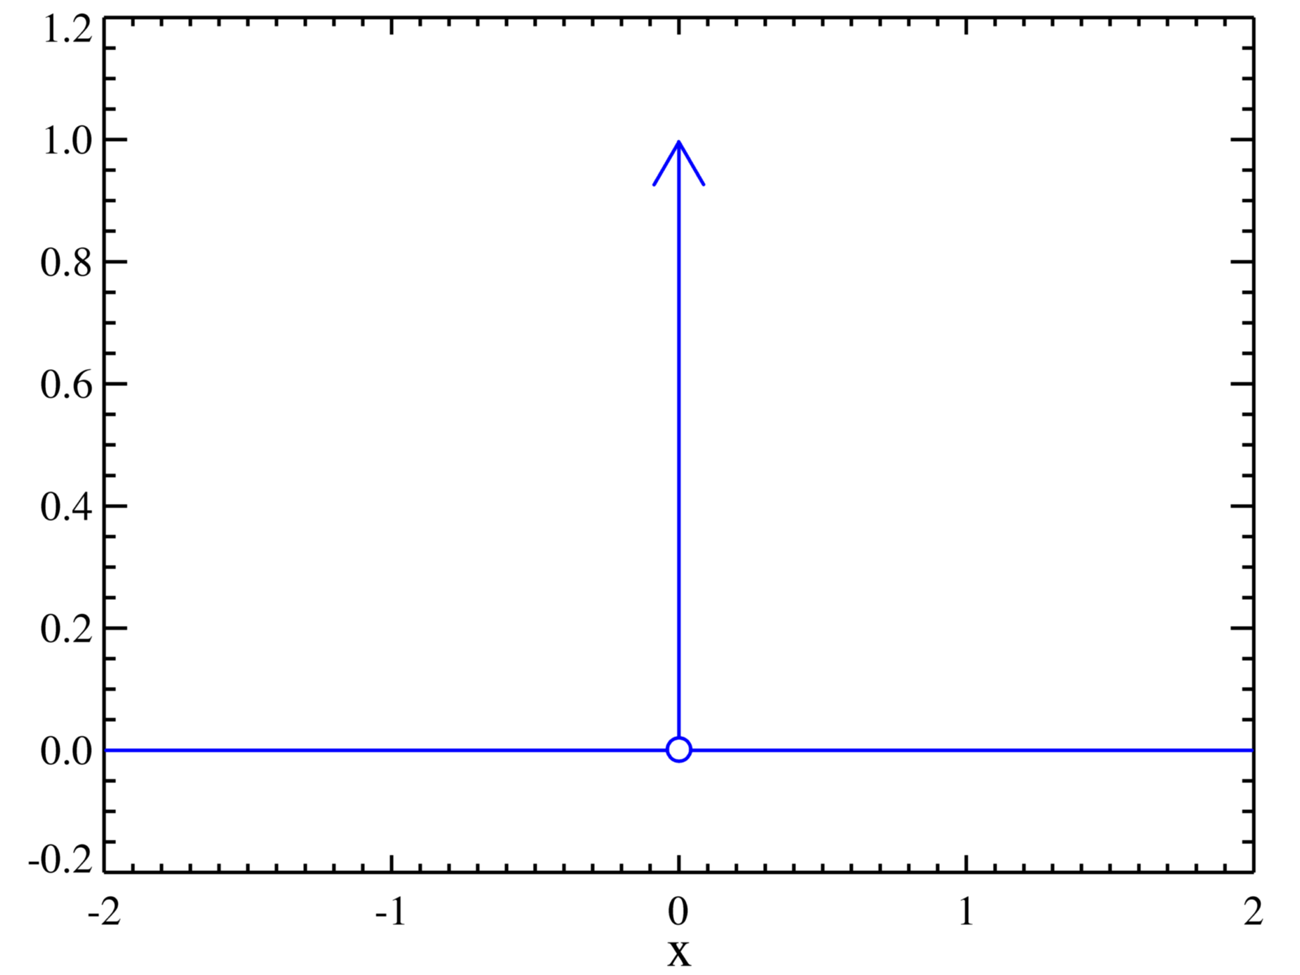
\includegraphics[scale = 0.2]{Dirac_distribution_PDF.png}
\end{figure}  

\footnote{Wikipedia - Delta di Dirac}

La Delta di Dirac gode di queste proprietà: 

{
    \Large 
    \begin{equation}
        \begin{cases}
            \delta (t = 0) = \infty \\ \\
            \delta (t \not = 0) = 0 \\ \\
            \int_{- \infty}^{ \infty} \delta (t) dt = 1
        \end{cases}
    \end{equation}
}

$\int_{- \infty}^{ \infty} \delta (t) dt = 1$ indica che l'area della Delta di Dirac è unitaria. \newline 

Se l'area è diversa da uno, basta moltiplicare la Delta di Dirac per un coefficiente moltiplicativo A. \newline 

La Delta di Dirac può trovarsi anche in un istante diverso da zero: 

{
    \Large 
    \begin{equation}
        t_0 \not = 0 
        \rightarrow 
        \delta (t - t_0)
     \end{equation}
}

o, in altri termini, possiamo vederla come una delta di Dirac shiftata nel tempo $t_0$. \newline 

Grazie alla Delta di Dirac shiftata nel tempo $t_0$, possiamo svolgere un campionamento ideale di un segnale s(t) all'instante $t_0$ come: 

{
    \Large 
    \begin{equation}
        \int_{- \infty}^{\infty} 
        s(t) \delta (t - t_0) dt 
        = 
        s(t_0)
    \end{equation}
}